\documentclass[journal]{IEEEtran}
\usepackage{lipsum} % 示例中使用的假文宏包
\ifCLASSINFOpdf
\else
   \usepackage[dvips]{graphicx}
\fi
\usepackage{url}

\hyphenation{op-tical net-works semi-conduc-tor}
\usepackage{pdfpages} % 添加pdfpages宏包
\usepackage{graphicx}
\usepackage{xcolor}

\begin{document}
\title{\color[rgb]{0,0.6,1}Digital Signal Processing Course Laboratory Experiments2 Report (October 2023)}

\author{12110405   Zhewei Chen}
%\thanks{This paragraph of the first footnote will contain the date on which you submitted your paper for review. It will also contain support information, including sponsor and financial support acknowledgment. For example, ``This work was supported in part by the U.S. Department of Commerce under Grant BS123456.'' }
%\thanks{The next few paragraphs should contain the authors' current affiliations, including current address and e-mail. For example, F. A. Author is with the National Institute of Standards and Technology, Boulder, CO 80305 USA (e-mail: author@boulder.nist.gov).}
%\thanks{S. B. Author, Jr., was with Rice University, Houston, TX 77005 USA. He is now with the Department of Physics, Colorado State University, Fort Collins, CO 80523 USA (e-mail: author@lamar.colostate.edu).}}

\markboth{EE323 Digital Signal Processing}
{Shell \MakeLowercase{\textit{et al.}}: Bare Demo of IEEEtran.cls for IEEE Journals}
\maketitle

\begin{abstract}
   This lab report introduces and investigates the basic concepts, representations and properties of discrete time systems. Using MATLAB to implement several discrete time systems and research their properties.
\end{abstract}

\begin{IEEEkeywords}
   discrete-time systems, difference equations, MATLAB
\end{IEEEkeywords}


\IEEEpeerreviewmaketitle



\section{Introduction}
\IEEEPARstart{T}{his} report is about Lab 2, focusing on the topic of discrete-time systems. The objective of the experiment is to learn the concepts and properties of discrete-time systems, understand the principles of discrete-time signal processing, and deepen the understanding of discrete-time systems through practical operation and analysis using MATLAB. We started by introducing the concept of discrete-time systems and discussed their importance and practical applications. We also analyzed the properties of discrete-time systems. In the background exercise section of the experiment, we designed integral and derivative discrete-time systems by selecting appropriate difference equations or block diagrams. We studied a difference equation case in the stock market. Next, we write MATLAB functions to implement integral and derivative discrete-time systems and study their properties. In the following stage, we design two types of discrete-time filters, test their impulse responses, and filter an audio signal. We then attempt to create the inverse system of one of the filters and validate it. Subsequently, we investigate the properties of the systems and perform comparative tests. Finally, we apply the filters to stock market data to analyze the properties.





\section{Experimental Contents}
\label{sec:guidelines}


\subsection{Breif Introduction of Discrete-Time Systems}



\subsection{Background Exercises}
Figures compiled of more than one sub-figure presented side-by-side, or 
stacked. If a multipart figure is made up of multiple figure
types 

 \begin{figure}[htbp]
   \centering
   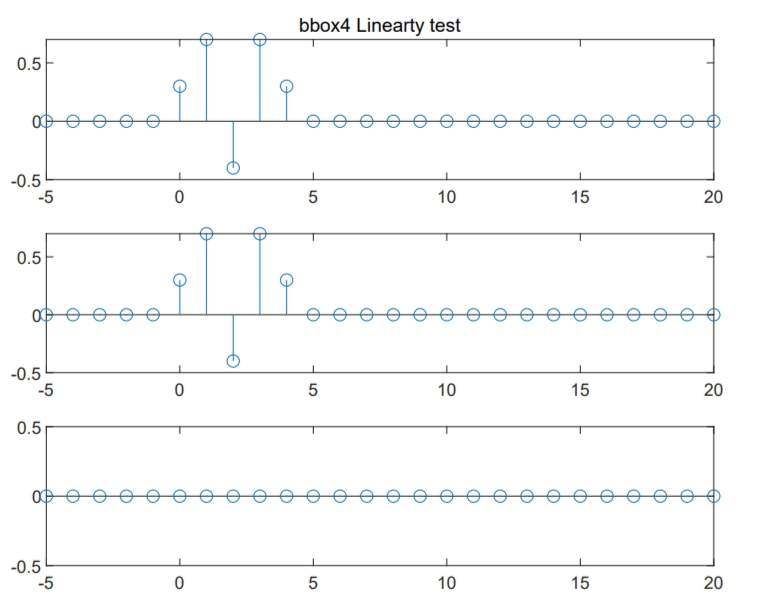
\includegraphics[width=0.5\textwidth]{bbox4 linear.png} % 将"your_image.png"替换为您的PNG图片文件名
   \caption{bbox4 linearity test by inputs signal $x[n]=\delta[n]$ and $x[n]=u[n]$}
   \label{fig:example}
 \end{figure}
 (one part is lineart, and another is grayscale or color) the figure 
should meet the stricter guidelines.







\subsection{Example Discrete-Time Systems}
Most charts, graphs, and tables are one column wide (3.5 inches/88 
millimeters/21 picas) or page wide (7.16 inches/181 millimeters/43 
picas). The maximum depth a graphic can be is 8.5 inches (216 millimeters/54
picas). When choosing the depth of a graphic, please allow space for a 
caption. Figures can be sized between column and page widths if the author 
chooses, however it is recommended that figures are not sized less than 
column width unless when necessary. 

\subsection{Difference Equations}

\subsection{Audio Filtering}
\subsection{Audio Filtering}
\subsection{Systems }
\subsection{Stock Market Example}
\section{Conclusion}

A conclusion section is not required. Although a conclusion may review the main points of the paper, do not replicate the abstract as the conclusion. A conclusion might elaborate on the importance of the work or suggest applications and extensions. 



\end{document}
